\documentclass[../main.tex]{subfiles}
\begin{document}
\section{Dependencia entera. Clausura entera.}
\begin{definition}
Sean $A\subset B$ dos anillos. Diremos que un elemento $x\in B$ es \textit{entero sobre $A$} si es raíz de un polinomio mónico con coeficientes en $A$, es decir, si satisface una ecuación de la forma
\begin{equation}\label{eq:depent}
    x^n+a_1x^{n-1}+\cdots+a_n=0
\end{equation}
donde $a_i\in A$ para toda $i\in\{1,\dots,n\}.$ Si todo $x\in B$ es entero sobre $A$, entonces decimos que $B$ es una \textit{extensión entera} de $A$
\end{definition}

\begin{definition}Diremos que un $A$-módulo $M$ es \textit{fiel}\footnote{Seguimos la traducción del Atiyah para \emph{faithful module}} si, dado $a\in A\setminus\{0\}$, existe $x\in M$ ral que $ax\neq 0$, esto es, $\anul_A(M)=\{0\}.$
\end{definition}

\begin{proposition}\label{prop:entcarac}Las siguientes afirmaciones son equivalentes.
\begin{itemize}
    \item[i)] $x\in B$ es entero sobre $A.$
    \item[ii)] $A[x]$ es un $A$-módulo finitamente generado.
    \item[iii)] $A[x]$ está contenido en un subanillo $C$ de $B$ finitamente generado como $A$-módulo.
    \item[iv)] Existe un $A[x]$-módulo \emph{fiel} $M$ que es finitamente generado como $A$-módulo.
\end{itemize}
\end{proposition}
\begin{proof}
$i)\Rightarrow ii)$ Para todo $r\neq0$, si sustituimos $x^r$  en (\ref{eq:depent}) obtenemos
$$x^{n+r}=-(a_1x^{n+r-1}+\cdots+a_nx^r)$$
Recursivamente podemos sustituir todas las potencias $\geq n$ por una expresión dependiente solo de las potencias $x^k$ con $k\<n$, y así todas las potencias de $x$ pertenecen al $A$-módulo $\langle 1,x,\dots,x^{n-1}\rangle_A$, por lo que $A[x]$ está generado como $A$-módulo por $\{1,x,\dots,x^{n-1}\}.$

$ii)\Rightarrow iii)$ Basta tomar $C=A[x].$

$iii)\Rightarrow iv)$ Análogamente, basta tomar $M=C.$

$iv)\Rightarrow i)$ Para esta implicación haremos uso del lema de Cayley-Hamilton. Sea $\phi:M\rightarrow M$, $m\mapsto xm$ y $\af:= A.$ Así, como $M$ es fiel, $\{0\}\neq xM\subseteq M$ y existen $a_i\in A$ de forma que
$$\phi^n+a_1\phi^{n-1}+\cdots+a_n\equiv 0,$$
y particularizando para $\phi(1_A) = x$ tenemos
$$x^n+a_1x^{n-1}+\cdots+a_n= 0$$
y $x$ es entero.
\end{proof}

\begin{corollary}
Sean $\{x_i\}_{i=1}^n\subset B$ elementos enteros sobre $A.$ Se tiene que el anillo $A[x_1,\dots,x_n]$ es un $A$-módulo finitamente generado.
\end{corollary}

\begin{corollary}
El conjunto de los elementos enteros de $B$ sobre $A$ es un subanillo de $B$ que contiene a $A.$
\end{corollary}

\begin{proof}
Denotemos por $C$ al conjunto definido en el corolario y tomemos $x,y\in C$. Sabemos que $A[x,y]$ es un $A$-módulo finitamente generado. Como $A[x\pm y],A[xy]\subset A[x,y]$, por $iii)$ de \ref{prop:entcarac} se tiene que $x\pm y$ como $xy$ son enteros sobre $A$.
\end{proof}

\begin{definition}
Sean $A\subset B$ dos anillos, el anillo $\overline{A}^B$ de los elementos enteros de $B$ sobre $A$ se llama \textit{clausura entera} del anillo $A$ en $B$. Si $A=\overline{A}^B$, se dice que  $A$ es \textit{íntegramente cerrado} en $B$. Si $\overline{A}^B = B$, se dice que $B$ es \textit{entero} sobre $A$.
\end{definition}

\begin{corollary}[Transitividad de la dependencia entera] Si $A\subseteq B\subseteq C$ son anillos, $B$ es entero sobre $A$ y $C$ es entero sobre $B$, entonces $C$ es entero sobre $A.$
\end{corollary}

\begin{corollary}
Sean $A\subseteq B$ anillos. $\overline{A}^B$ es íntegramente cerrado sobre $B.$
\end{corollary}

\begin{proposition}\label{props_entera}Sea $A\subseteq B$ una extensión entera.
\begin{itemize}
    \item[i)] Si $B$ es un cuerpo, entonces $A$ es un cuerpo.
    \item[ii)] Si $A$ es un cuerpo y $B$ un dominio de integridad, entonces $B$ es un cuerpo.
    \item[iii)] Sean $\mathfrak{b}$ un ideal de $B$ y $\af:=\mathfrak{b}\cap A$, entonces $A/\af\hookrightarrow B/\mathfrak{p}$ es una extensión entera\footnote{En este caso, se entiende que los elementos de $B/\mathfrak{b}$ han de cumplir una ecuación con coeficientes en la imagen de $A/\mathfrak{p} = A/\mathfrak{q}$. En verdad esto es equivalente a pensar en términos de $A/\af$ módulos como en la proposición \ref{prop:entcarac}, porque el producto externo es $(a+\af)(b+\mathfrak{b}) =(a+\mathfrak{b})(b+\mathfrak{b}) = ab \mathfrak{b} $}.
    \item[iv)] Sea $S\subset A$ un conjunto mult. cerrado. El $S^{-1}A$-módulo $S^{-1}B$ es un anillo y $S^{-1}A\hookrightarrow S^{-1}B$ es una extensión entera.
\end{itemize}
\end{proposition}
\begin{proof}
\textit{i)} Dado $a\in A\setminus\{0\}$, existe $b\in B $ tal que $ab=1.$ Además,
$$b^n+a_1b^{n-1}+\cdots+a_n=0$$
para ciertos $a_i\in A.$ Multiplicando la ecuación anterior por $a^n$ resulta:
$$1+a_1a+\cdots+a_na^n=0\Longleftrightarrow a(-a_1-\cdots-a_na^{n-1})=1.$$

\textit{ii)} Sea  $b\in B\setminus\{0\}.$ De nuevo, tenemos una ecuación de la forma
$$b^n+a_1b^{n-1}+\cdots+a_n=0$$
para ciertos $a_i\in A.$ Como $B$ es DI, se tiene $a_n\neq0.$ Por hipótesis existe $a\in A$ de forma que $aa_n=1$ y, multiplicando la ecuación por este elemento, obtenemos de forma análoga al caso anterior un inverso para elemento $b.$

\textit{iii)} Sea $x\in B$ que es entero sobre $A$ y por tanto cumple una ecuación $x^n+a_1x^{n-1}+\cdots+a_n=0$ con $a_i \in A$. Tomamos clases módulo $\mathfrak{b}$ y observamos que $a_i+ \mathfrak{a}+ \af \mapsto a_i +\mathfrak{b}$.

\textit{iv)} Es claro que la aplicación es inyectiva. Sea $s\in S$ y $b\in B$ y una ecuación
$$b^n+a_1b^{n-1}+\cdots+a_n=0$$
para ciertos $a_i\in A.$ En $S^{-1}B$ multiplicamos por $\frac{1}{s^n}$ y tenemos la ecuación
$$\frac{b^n}{s^n}+\frac{a_1}{s}\frac{b^{n-1}}{s^{n-1}}+\cdots+\frac{a_n}{s^n}=0.$$
\end{proof}

\begin{lemma}\label{lemma:idext}
Sean $A\subset B$ una extensión entera y $\af\subset A$ un ideal, entonces la clausura del ideal $\overline{\af}^B$ \footnote{Los $b\in B$ enteros con coeficientes en $\mathfrak{a}$} coincide con $\sqrt{\af B}$. Además, $\sqrt{\af B}\cap A=\sqrt{\af}.$
\end{lemma}
\begin{proof}
Por un lado, si $b\in B$ tiene una ecuación de la forma (\ref{eq:depent}), por lo tanto $b^n\in\af B$ y así $b\in\sqrt{\af B}$. Recíprocamente, si $b\in\sqrt{\af B}$, existe $r\in\N$ tal que $b \in \af B$ y se escribirá tal que $b^r=\sum_{i=1}^sb_i\alpha_i$ para ciertos $b_i \in B$ y $\alpha_i \in \af$.
Los elementos $b_i$ son enteros sobre $A$; así, $C:=A[b_1,\dots,b_s]$ es un $A$-módulo finitamente generado que contiene a $b^r$, en particular, $b^r\in\af C$. Vamos a aplicar Cayley-Hamilton: consideremos el homomorfismo de $A$-módulos $\phi: C\rightarrow C$ definida por $c\mapsto b^r c$, cuya imagen está contenida en $\af C$. Por Cayley existen $a_i\in\af$ tales que
$$\phi^n+a_1\phi^{n-1}+\cdots+a_{n-1}\phi+a_n\equiv 0.$$
y evaluando en $1\in C$ resulta
$$(b^r)^n+a_1(b^r)^{n-1}+\cdots+a_{n-1}(b^r)+a_n= 0$$
luego $b^r$ es entero con coeficientes en $\af$.

Por último, si $x\in\sqrt{\af}$, existe $n\in\N$ tal que $x^n\in\af$, es decir, $x^n\in\sqrt{\af B}.$
\end{proof}

\begin{definition}
En las condiciones del lema anterior, se dice que los elementos $x\in\sqrt{\af B}$ dependen íntegramente del ideal $\af.$
\end{definition}

Recordamos del capítulo 3 que dado un dominio de integridad A, el anillo de fracciones $S^{-1}A$ con $S = A \setminus \operatorname{Div}_0A = A\setminus \{0\}$ es el cuerpo de fracciones (el menor cuerpo que contiene a $A$). Denotemos este cuerpo por $K_A.$

\begin{definition}
Diremos que un anillo $A$ es \textit{íntegramente cerrado} si lo es sobre su cuerpo de fracciones $K_A$, es decir, si $A=\overline{A}^{K_A}.$
\end{definition}

\begin{lemma}
Si $A$ es DFU, entonces es íntegramente cerrado en su cuerpo de fracciones: $A=\overline{A}^{K_A}$.
\end{lemma}
\begin{proof}
Hay que probar que todo elemento entero de $K_A$ es un elemento de $A$. Sea $\frac{a}{b}$ es entero sobre $A$, como $A$ es DFU podemos expresarlo como cociente de dos elementos coprimos. Es raíz de un polinomio mónico con coeficientes en $A$, así por el teorema \ref{rational_root} (de la raíz racional) $b$ divide a $1$, luego es una unidad y así $\frac{a}{b} = \frac{ab^{1}b}{b} = ab^{-1}\in A$.
\end{proof}

\begin{corollary}
Todo anillo de polinomios sobre un cuerpo es cerrado sobre su cuerpo de fracciones.
\end{corollary}

\begin{proposition}\label{prop:polmin}
Sean $A$ y $B$ dominios de integridad, $A$ íntegramente cerrado sobre $B$ y $A\subset B$ extensión entera. Para cada $b\in B$, $b$ es entero sobre $K_A$ y su polinomio mínimo sobre $K_A$ tiene coeficientes en $A$. Si además es entero sobre un ideal $\af$ de $A$, el polinomio mínimo de $b$ sobre $K_A$ tiene sus coeficientes sobre $\sqrt{\af}.$
\end{proposition}

\begin{proof}
Lo probamos para un ideal $\af$ de $A$ posiblemente impropio. Si $b$ es entero sobre $\af$, lo es sobre $K_A$ sin más que tomar el polinomio mónico coeficientes en $\af \subset K_A$.

Sean $P(T)\in K_A[T]$ su polinomio mínimo y $L\supset K_A$ un cuerpo donde $P(T)$ descompone en factores lineales. Estas raíces serán por tanto elementos de $L$ enteros sobre $\af.$ Por el teorema de las funciones simétricas elementales, los coeficientes de $P(T)$, que pertenecen a $K_A$, son sumas y productos de elementos de $L$ enteros sobre $\af$; es decir, los coeficientes de $P(T)$ pertenecen a $\overline{\af}^{K_A}=\af.$

Por el lema \ref{lemma:idext} resulta que los coeficientes de $P(T)$ pertenecen a
$$\overline{a}^{K_A}\cap A=\sqrt{\af K_A}\cap A=\sqrt{\af}.$$
\end{proof}

\section{Teoremas del ascenso y del descenso (\textit{going-up} y \textit{going-down}}
Los dos teoremas abordan el problema siguiente: dada una extensión $A\to B$, una cadena $p_0 \subsetneq \p_1 \subsetneq \dots \subsetneq \p_n$ (respectivamente en sentido descendente para la inclusión) de ideales primos en $A$, y una cadena $\q_0 \subsetneq \q_1 \subsetneq \dots \subsetneq \q_m$ con $m<n$ (resp. $\supsetneq$) de primos en $B$ tales que $\q_i^c = \p_i$,
¿puede completarse la cadena de $B$ con ideales primos $\q_{m+1}\subsetneq \subsetneq \q_n$ (resp. $\supsetneq$) de forma que $\q_i^c = \p_i$? Los nombres \textit{going-up} y \textit{going-down} se refieren al sentido de la cadena. Como veremos, para la versión descendente hay que pedir más requisitos que para la ascendente.

\begin{proposition}\label{prop:lying} Sea $A\subset B$ una extensión entera.
\begin{itemize}
    \item[i)] Un $\q\in\Spec B$ es maximal si y solo si $\p:=\q\cap A$  es maximal.
    \item[ii)] Dados $\q_1,\q_2\in\Spec B$, si $\q_1\subset\q_2$ y $\q_1\cap A=\q_2\cap A=\p$, entonces $\q_1=\q_2.$
    \item[iii)] Para todo ideal primo $\mathfrak{p}$ de $A$, existe un primo $\mathfrak{q}$ en $B$ tal que $\mathfrak{p} = \mathfrak{q} \cap A$ (la contracción $\Spec B\rightarrow\Spec A$ es suprayectiva).
\end{itemize}
\end{proposition}

\begin{proof}
\textit{(i)} Sabemos por la proposición \ref{props_entera} que $A/\p \subset B/\q$ es una extensión entera. Como $\q$ es maximal $B/\q$ es cuerpo y, por la misma proposición, $A/\p$ también lo es y por tanto $\p$ es maximal. Recíprocamente, si $\p$ es maximal, $A/\p$ y como $B/\q$ es DI porque $\q$ es primo, de nuevo la proposición nos dice que $B/\q$ es cuerpo, luego $\q$ maximal.

\textit{(ii)} Por proposición anterior, $B_\p$\footnote{Es notación, no podemos considerar la localización de $B$ en $\p$ en sentido clásico, esto es, $S = B \setminus \mathfrak{p}$ y $B_\p = S^{-1}B$, porque no sabemos si es un ideal primo en $B$. Lo que hacemos es denotar así a $S^{-1}B$ donde $S= A\setminus \p$ que sí es un conjunto multiplicativamente cerrado y como indica la proposición \ref{props_entera} es extensión de $A_\p$.} es extensión entera sobre $A_\p.$ Tenemos que $\p^e$ es el único ideal maximal de $A_\p$, como $\q_1^e\subseteq \q_2^e$ y $\q_1^{ec}= \q_2^{ec}=\p$, el apartado anterior nos dice que $\q_1^e$ y $\q_2^e$ son maximales; es decir, $\q_1^e=\q_2^e.$ Así, $\q_1=\q_1^{ec}=\q_2^{ec}=\q_2.$

\textit{(iii)} Como antes, $B_\p$ es entero sobre $A_\p$ y el diagrama de la Figura \ref{pre_going_up} es conmutativo. Sea $\mathfrak{n}$ un ideal maximal de $B_\p.$
Se tiene así que $\mathfrak{m}:=\mathfrak{n}\cap A_\p$ es maximal y, por lo tanto, $\mathfrak{m}=\p^e.$ Si $\q=\beta^{-1}(\mathfrak{n})$, entonces $\q$ es primo y $\q\cap A=\alpha^{-1}(\mathfrak{m})=\p$ por la conmutatividad del diagrama.

\begin{figure}
  \centering


  \tikzset{every picture/.style={line width=0.75pt}} %set default line width to 0.75pt

  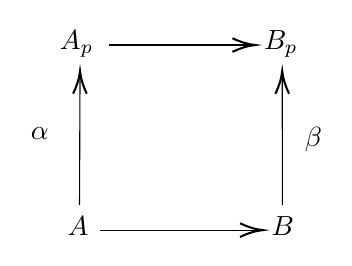
\begin{tikzpicture}[x=0.75pt,y=0.75pt,yscale=-1,xscale=1]
  %uncomment if require: \path (0,300); %set diagram left start at 0, and has height of 300


  % Text Node
  \draw (272.67,152.4) node [anchor=north west][inner sep=0.75pt]    {$A$};
  % Text Node
  \draw (371,152.4) node [anchor=north west][inner sep=0.75pt]    {$B$};
  % Text Node
  \draw (269,62.73) node [anchor=north west][inner sep=0.75pt]    {$A_{\mathfrak{p}}$};
  % Text Node
  \draw (367.33,62.73) node [anchor=north west][inner sep=0.75pt]    {$B_{\mathfrak{p}}$};
  % Text Node
  \draw (255,109.4) node [anchor=north west][inner sep=0.75pt]    {$\alpha $};
  % Text Node
  \draw (387,109.4) node [anchor=north west][inner sep=0.75pt]    {$\beta $};
  % Connection
  \draw    (289.67,160) -- (366,160) ;
  \draw [shift={(368,160)}, rotate = 180] [color={rgb, 255:red, 0; green, 0; blue, 0 }  ][line width=0.75]    (10.93,-3.29) .. controls (6.95,-1.4) and (3.31,-0.3) .. (0,0) .. controls (3.31,0.3) and (6.95,1.4) .. (10.93,3.29)   ;
  % Connection
  \draw    (279.71,148) -- (279.95,85.33) ;
  \draw [shift={(279.95,83.33)}, rotate = 450.21] [color={rgb, 255:red, 0; green, 0; blue, 0 }  ][line width=0.75]    (10.93,-3.29) .. controls (6.95,-1.4) and (3.31,-0.3) .. (0,0) .. controls (3.31,0.3) and (6.95,1.4) .. (10.93,3.29)   ;
  % Connection
  \draw    (294,70.83) -- (362.33,70.83) ;
  \draw [shift={(364.33,70.83)}, rotate = 180] [color={rgb, 255:red, 0; green, 0; blue, 0 }  ][line width=0.75]    (10.93,-3.29) .. controls (6.95,-1.4) and (3.31,-0.3) .. (0,0) .. controls (3.31,0.3) and (6.95,1.4) .. (10.93,3.29)   ;
  % Connection
  \draw    (377.48,148) -- (377.36,85.33) ;
  \draw [shift={(377.36,83.33)}, rotate = 449.89] [color={rgb, 255:red, 0; green, 0; blue, 0 }  ][line width=0.75]    (10.93,-3.29) .. controls (6.95,-1.4) and (3.31,-0.3) .. (0,0) .. controls (3.31,0.3) and (6.95,1.4) .. (10.93,3.29)   ;

  \end{tikzpicture}
  \label{pre_going_up}
  \caption{}
\end{figure}
\end{proof}

\begin{theorem}[\textbf{del ascenso (Going-up)}]
Sea $A\subseteq B$ una extensión entera, $\p_0\subset\p_1$ primos de $A$ y $\q_0\in\Spec B$ tal que $\q_0\cap  A=\p_0.$ Entonces existe $\q_1\in\Spec B$ tal que $\q_0\subset\q_1$ tal que $\q_1\cap A=\p_1.$
\end{theorem}
\begin{figure}
  \centering
  \tikzset{every picture/.style={line width=0.75pt}} %set default line width to 0.75pt

  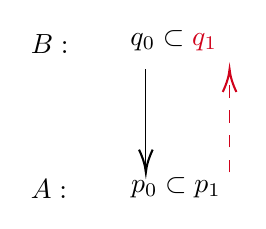
\begin{tikzpicture}[x=0.75pt,y=0.75pt,yscale=-1,xscale=1]
  %uncomment if require: \path (0,300); %set diagram left start at 0, and has height of 300

  %Straight Lines [id:da8639627348676742]
  \draw    (319.8,50.7) -- (319.8,98.37) ;
  \draw [shift={(319.8,100.37)}, rotate = 270] [color={rgb, 255:red, 0; green, 0; blue, 0 }  ][line width=0.75]    (10.93,-3.29) .. controls (6.95,-1.4) and (3.31,-0.3) .. (0,0) .. controls (3.31,0.3) and (6.95,1.4) .. (10.93,3.29)   ;
  %Straight Lines [id:da07580641488983964]
  \draw [color={rgb, 255:red, 208; green, 2; blue, 27 }  ,draw opacity=1 ] [dash pattern={on 4.5pt off 4.5pt}]  (360.13,100.37) -- (360.13,52.7) ;
  \draw [shift={(360.13,50.7)}, rotate = 450] [color={rgb, 255:red, 208; green, 2; blue, 27 }  ,draw opacity=1 ][line width=0.75]    (10.93,-3.29) .. controls (6.95,-1.4) and (3.31,-0.3) .. (0,0) .. controls (3.31,0.3) and (6.95,1.4) .. (10.93,3.29)   ;

  % Text Node
  \draw (311.47,101.6) node [anchor=north west][inner sep=0.75pt]    {$\mathfrak{p}_{0} \subset \mathfrak{p}_{1}$};
  % Text Node
  \draw (263.13,102.6) node [anchor=north west][inner sep=0.75pt]    {$A:$};
  % Text Node
  \draw (311.13,30.93) node [anchor=north west][inner sep=0.75pt]    {$\mathfrak{q}_{0} \subset \textcolor[rgb]{0.82,0.01,0.11}{\mathfrak{q}_{1}}$};
  % Text Node
  \draw (263.13,32.6) node [anchor=north west][inner sep=0.75pt]    {$B:$};


  \end{tikzpicture}
  \caption{Going-up}
\end{figure}

\begin{proof}
Sabemos que $A/\p_0\hookrightarrow B/\q_0$ es una extensión entera. El ideal $\p_1/\p_0$ es primo en $A/\p_0$
Por la proposición \ref{prop:lying} existe $\q_1/\q_0\in\Spec {B/\p_0}$  que se contrae a $\p_1/\p_0$, y así $\q_0 \subset \q_1$ y $\q_1\cap A=\p_1.$
\end{proof}

\begin{definition}
Dado un anillo $A$, se denomina \textit{dimensión de Krull de $A$},  $\dimk A$, al supremo de las longitudes de cadenas de ideales primos de la forma $\p_0\supsetneq\p_1\supsetneq\cdots\supsetneq\p_r$ con $\p_i\in\Spec A\}$, pudiendo ser infinito.
\end{definition}

\begin{corollary}
Dada una extensión entera $A\subset B$, $\dimk A=\dimk B.$
\end{corollary}

\begin{lemma}
Sea $\phi:A\rightarrow B$ un homomorfismo de anillos y definamos
$$\begin{array}{rrcl}
    \phi^*:&\Spec B&\rightarrow&\Spec{A}  \\
     &\q&\mapsto&\phi^{-1}(\q)
\end{array}.$$
Dado $\p\in\Spec A$, $\p$ es contraído de algún ideal $\q\in\Spec B$ si, y sólo si, $\p^{ec}=\p.$
\end{lemma}
\begin{proof}
($\Rightarrow$) Si existe $\q\in\Spec B$ tal que $\q^c=\p$, entonces $\p=\q^c=\q^{cec}=\p^{ec}$.

($\Leftarrow$) Tomamos $S:=A\setminus\p$ y $S':=\phi(S)\subset B$ que es multiplicativamente cerrado. La apliación $\delta_{S'}\circ \phi: A \to S^{-1}B$ lleva elementos de $S$ unidades de $S'^{-1}B$ (elementos de $S'$), luego por la propiedad universal del anillo de fracciones existe un homomorfismo $\Phi:S^{-1}A\rightarrow S'^{-1}B$ que hace conmutativo el diagrama \ref{anillosfraccionesuniversal}
\begin{figure}
  \tikzset{every picture/.style={line width=0.75pt}} %set default line width to 0.75pt
  \centering
  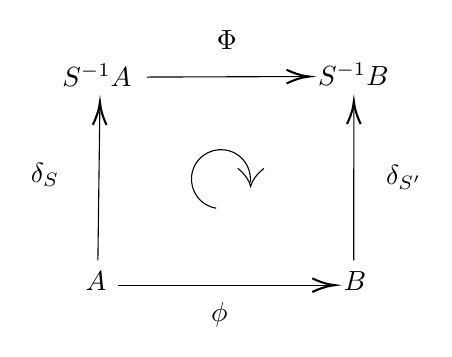
\begin{tikzpicture}[x=0.75pt,y=0.75pt,yscale=-1,xscale=1]
  %uncomment if require: \path (0,300); %set diagram left start at 0, and has height of 300

  %Shape: Arc [id:dp0994638953215361]
  \draw  [draw opacity=0] (361.51,112.73) .. controls (359.92,112.47) and (358.34,111.93) .. (356.85,111.09) .. controls (350.01,107.25) and (347.58,98.59) .. (351.42,91.75) .. controls (355.26,84.91) and (363.91,82.48) .. (370.76,86.32) .. controls (375.87,89.18) and (378.52,94.75) .. (377.93,100.23) -- (363.8,98.7) -- cycle ; \draw   (361.51,112.73) .. controls (359.92,112.47) and (358.34,111.93) .. (356.85,111.09) .. controls (350.01,107.25) and (347.58,98.59) .. (351.42,91.75) .. controls (355.26,84.91) and (363.91,82.48) .. (370.76,86.32) .. controls (375.87,89.18) and (378.52,94.75) .. (377.93,100.23) ;
  \draw   (384.46,93.57) .. controls (380.95,96.44) and (378.82,99.31) .. (378.1,102.21) .. controls (377.44,99.3) and (375.38,96.37) .. (371.93,93.44) ;

  % Text Node
  \draw (297.36,142.2) node [anchor=north west][inner sep=0.75pt]    {$A$};
  % Text Node
  \draw (421.76,142.2) node [anchor=north west][inner sep=0.75pt]    {$B$};
  % Text Node
  \draw (286.16,42) node [anchor=north west][inner sep=0.75pt]    {$S^{-1} A$};
  % Text Node
  \draw (409.36,41.6) node [anchor=north west][inner sep=0.75pt]    {$S^{-1} B$};
  % Text Node
  \draw (360.56,26) node [anchor=north west][inner sep=0.75pt]    {$\Phi $};
  % Text Node
  \draw (270.96,89.6) node [anchor=north west][inner sep=0.75pt]    {$\delta _{S}$};
  % Text Node
  \draw (442.16,91) node [anchor=north west][inner sep=0.75pt]    {$\delta _{S'}$};
  % Text Node
  \draw (357.76,156.8) node [anchor=north west][inner sep=0.75pt]    {$\phi $};
  % Connection
  \draw    (314.36,149.8) -- (416.76,149.8) ;
  \draw [shift={(418.76,149.8)}, rotate = 180] [color={rgb, 255:red, 0; green, 0; blue, 0 }  ][line width=0.75]    (10.93,-3.29) .. controls (6.95,-1.4) and (3.31,-0.3) .. (0,0) .. controls (3.31,0.3) and (6.95,1.4) .. (10.93,3.29)   ;
  % Connection
  \draw    (304.52,137.8) -- (305.48,63.6) ;
  \draw [shift={(305.5,61.6)}, rotate = 450.74] [color={rgb, 255:red, 0; green, 0; blue, 0 }  ][line width=0.75]    (10.93,-3.29) .. controls (6.95,-1.4) and (3.31,-0.3) .. (0,0) .. controls (3.31,0.3) and (6.95,1.4) .. (10.93,3.29)   ;
  % Connection
  \draw    (427.77,137.8) -- (427.85,63.2) ;
  \draw [shift={(427.85,61.2)}, rotate = 450.06] [color={rgb, 255:red, 0; green, 0; blue, 0 }  ][line width=0.75]    (10.93,-3.29) .. controls (6.95,-1.4) and (3.31,-0.3) .. (0,0) .. controls (3.31,0.3) and (6.95,1.4) .. (10.93,3.29)   ;
  % Connection
  \draw    (328.16,49.53) -- (404.36,49.28) ;
  \draw [shift={(406.36,49.27)}, rotate = 539.81] [color={rgb, 255:red, 0; green, 0; blue, 0 }  ][line width=0.75]    (10.93,-3.29) .. controls (6.95,-1.4) and (3.31,-0.3) .. (0,0) .. controls (3.31,0.3) and (6.95,1.4) .. (10.93,3.29)   ;

  \end{tikzpicture}
  \label{anillosfraccionesuniversal}
  \caption{}
\end{figure}
Veamos ahora que $\p$ extendido a $S'^{-1}B$ es un ideal propio. En caso contrario, $1_B\in \p S'^{-1}B$, i.e., $1_B=\sum\phi(p_i)\frac{b_i}{\phi(s_i)}.$ Llamando $s'.=\prod\phi(s_i)$ y $s'=\sum\phi(p_i)b_i'$, tenemos $s'\in \p B$ y $\prod s_i\in \p^{ec}=\p$ y $s_i\in S$, pero esto es absurdo.

Por ser propio, existe $\mathfrak{m}\subset S'^{-1}B$ maximal tal que $\mathfrak{m}\supset \p S'^{-1}B.$ $\Phi^{-1}(\mathfrak{m})$ es un ideal propio que necesariamente está contenido en $\p S^{-1}A$ por ser éste el único ideal maximal. Por otra parte, dado $\frac{p}{s}\in\p S^{-1}A$, $\frac{\phi(p)}{\phi(s)}\in\p S'^{-1}B\subset \mathfrak{m}$ y $\phi(\frac{p}{s})\in\mathfrak{m}$; es decir, $\frac{p}{s}\in\Phi^{-1}(\mathfrak{m)}.$ Con todo $\Phi^{-1}(m)=\p S^{-1}A.$

Como el único ideal de $S^{-1}A$ que yace sobre $\p$ es $\p S^{-1}A$, también $\mathfrak{m}$ yace sobre $\p.$ Por último, $\delta'^{-1}(\mathfrak{m})$ es un ideal primo propio que por la conmutatividad del diagrama yace sobre $\p.$
\end{proof}

\begin{theorem}[\textbf{Going-down}] Sea $A\subset B$ una extensión entera donde $A$ y $B$ son dominios de integridad y $A$ es íntegramente cerrado. Sean $\p_0,\p_1\in\Spec A$ y $\q_0\in\Spec B$ tales que $\p_0\supset\p_1$ y $\q_0\cap A=\p_0.$ Bajo estas hipótesis, existe $\q_1\in\Spec B$ tal que $\q_0\supset\q_1$ y $\q_1\cap A=\p_1.$
\end{theorem}

\begin{proof}
Sean $A\hookrightarrow A_{\p_0}\hookrightarrow B_{\q_0}$ y $A\hookrightarrow B\hookrightarrow B_{\q_0}$ homomorfismo de anillos, todos inyectivos por ser $A$ y $B$ dominios de integridad.

Sabemos que $\p_0^e=\q_0^{ce}\subset\q_0$ donde la contracción y extensión son de $A$ a $B$. Entonces tenemos $\p_1^e\subset\p_0^e\subset\q_0$ donde este último es primo, por tanto propio, y así el resto también son ideales propios.

Solo tenemos que probar que $\p_1^{ec} = \p_1$, donde la extensión-contracción es respecto a $A\to B_{\q_0}$ mediante el diagrama \ref{anillosfraccionesuniversal} es $\p_1$ (en otra notación $\p_1 B_{\q_0}\cap A=\p_1$).
Si demostramos esto, por el lema anterior existe un ideal primo de $B_{\q_0}$ que se contrae a $\p_1$; es decir, existe $\q_1\in\Spec B$ tal que $\q_1\subset\q_0$ y $\q_1B_{\q_0}\cap A=\p_1$, lo que implica que $\q_1\cap A=\p_1.$

Sea $x=\frac{y}{s}\in \p_1^{e}= \p_1B$, donde $y\in\p_1 B$ y $s\in B\setminus\q_0$. Como $\p_1B \subset \sqrt{\p_1B}$, el lema \ref{lemma:idext} tenemos que $y$ es entero sobre $\p_1$ y por la proposición \ref{prop:polmin}, el polinomio mínimo de $y$ sobre $K_A$ tiene coeficientes en $\p_1$
\begin{equation}\label{polmin_s}
  T^n+a_1T^{n-1}+\cdots+a_{n-1}T+a_n
\end{equation}

Si además $x\in A \subset K_A$, tomamos su inverso $x^{-1}\in K_A$ y entonces el polinomio mínimo de $s=yx^{-1}$ sobre $K_A$ es
$$T^n+v_1T^{n-1}+\cdots+v_{n-1}T+v_n$$
donde $v_i:=\frac{a_i}{x^i}$. Ahora bien, como $s\in B$ volvemos a estar en las hipótesis de la proposición \ref{prop:polmin} (esta vez en el caso general) y por lo tanto $v_i\in A.$ Por esto también $v_i x^i=a_i\in\p_1$, pero no todo $v_i\in\p_1$ pues, en caso contrario, sustituyendo $s$ en (\ref{polmin_s}) y despejando $s^n$, este pertenecería a $\p_1^e\subset \q_0$, lo que es absurdo porque $s\in B\setminus \q_0$.
Por tanto, para algún $i$ se tiene $x^i\in\p_1$ lo que implica por primalidad que $x\in \p_1$ como queríamos ver.
\end{proof}

\begin{definition}
Dado un anillo $A$ y un ideal $\p\in\Spec A$, definimos la \textit{altura de $\p$} y la denotamos por $\operatorname{ht}_A(\p)$ ó $\operatorname{ht}(\p)$ al valor
$$\sup\{r\in\N\ :\ \exists\p_0\supsetneq \cdots \supsetneq \p_r,\ \p_i\in\Spec A\}.$$
\end{definition}

\begin{remark}
Recordando que $\sup\{r\in\N\ :\ \exists\p_0\supsetneq \cdots \supsetneq \p_r,\ \p_i\in\Spec A\}=\dimk A$ se tiene que $\operatorname{ht}_A(\p)=\dimk A_\p.$
\end{remark}

Tras esta definición tenemos el siguiente corolario.

\begin{corollary}
Sean $A\subset B$ una extensión entera de dominios de integridad y $A$ íntegramente cerrado. Sea $\q\in\Spec B$ y $\p:=\q\cap A.$ Se tiene que $\operatorname{ht}_A(\p)=\operatorname{ht}_B(\q).$
\end{corollary}

\begin{proof}
Si $\q_1\subset\q_0\in\Spec B$, $\q_1\cap A=\q_0\cap A$
\end{proof}

\end{document}
